\documentclass[18pt,aspectratio=149]{beamer}
\usepackage[]{bookmark}
\usepackage[utf8]{inputenc}
\usepackage{amsmath}
\usepackage{amsfonts}
\usepackage{amssymb}
\usepackage{tikz}
\usepackage{xcolor}
\usepackage[dutch]{babel}
\usepackage{sansmathaccent}
\usepackage{graphicx}
\usepackage{pgfplots}

\usepackage[style=authoryear,backend=biber]{biblatex}

\addbibresource{bibliography3.bib} 
\pdfmapfile{+sansmathaccent.map}

\title{RMC voor lineaire ODEs}
\author{Isidoor Pinillo Esquivel }
\usetheme{Madrid}
\date{}

\begin{document}

% 1 min
\begin{frame}
    \titlepage
\end{frame}
% 2 min
\begin{frame}
    \frametitle{Mijn motivatie}
    Veralgemenen van WoS algoritme van (\cite{sawhney_grid-free_2022})
    naar tijd
    \vspace{-0.25cm}
    \begin{figure}[h!]
        \centering
        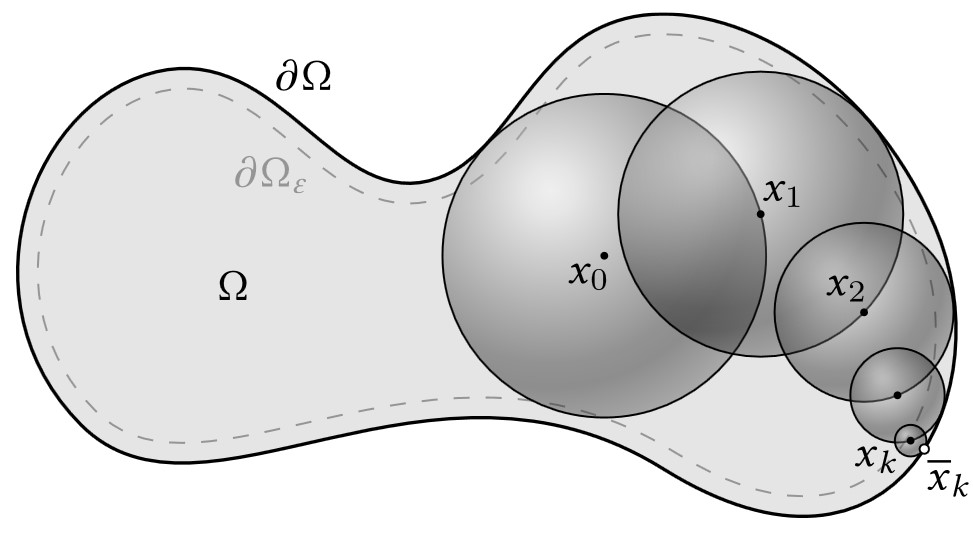
\includegraphics[width=0.6\textwidth]{imgs/Walk_on_Spheres_illustration.jpg}
        \label{fig:Walk_on_Spheres_illustration.jpg}
    \end{figure}
\end{frame}

\begin{frame}
    \frametitle{Overzicht}
    \begin{itemize}
        \item randomized information/sample-based complexity theory of summation
        \item main Poisson algoritme voor lineaire beginwaardeproblemen
        \item recursive first passage resampling as a U-estimator?
    \end{itemize}
\end{frame}


% 2 min
\begin{frame}
    \frametitle{Random sample efficientie van optelling}
    \action<+->{
        Probleem: benader $\bar{x} = \frac{1}{k}\sum_{i=1}^{k} x_{i}$ met $n<k$ van de $x_{i}$'s $\in [0,1]$\\
        (symmetrisch in $x_{i}$) \\
        \vspace{0.5cm}
    }
    \action<+->{
        Vertrouwensinterval kans $=1$  $\sim \frac{k-n}{k}= 1-\frac{n}{k}$ \\
        (worst case scenarios van de missende informatie liggen $\frac{1}{k}$ uit elkaar) \\
        \vspace{0.5cm}
    }
    \action<+->{
        Benader door te samplen met vervanging $\bar{x}  \cong \frac{1}{n}\sum_{i=1}^{n} x_{I_{i}}$\\
        (zonder vervanging is sneller maar niet onafhankelijk) \\
        \vspace{0.5cm}
    }
    \action<+->{
        Variantie = RMSE $\sim O\left(\frac{1}{\sqrt{n}}\right)$\\
        en ook vertrouwensintervallen kans $<1$\\
        (CLT of Chebychev's ongelijkheid)\footcitetext{heinrich_optimal_2001}\\
    }

\end{frame}

% 2 min
\begin{frame}
    \frametitle{Monte Carlo Integratie}
    Integratie $\approx$ sommatie, integreerbare $f: \mathbb{R} \rightarrow [0,1]$:
    \begin{align}
        \int_{0}^{1} f(s) ds & = E[f(U)]                                 \\
                             & \cong \frac{1}{n} \sum_{j=1}^{n} f(U_{j}) \\
        \text{met } U_{j}    & \sim \text{Uniform}(0,1)
    \end{align}
    % Sommatie en integratie hebben $1$-sample unbiased estimator.
\end{frame}

\begin{frame}
    \frametitle{Lineaire ODEs}
    \action<+->{
        Probleem: benader $y(t)$ waar $y'(t) = A(t)y(t)$ gegeven $y(0)$ en $A(t)$ begrensd\\
        \vspace{0.25cm}
    }
    \action<+->{
        Biased algoritme met $n$ samples
        \footcite{jentzen_random_2009},\footcite{daun_randomized_2011} \\
        (enkel random)\\
        \vspace{0.25cm}
    }
    \action<+->{
        $\nexists$ unbiased algoritme met $n$ samples van $A(t)$\\
        (niet bewezen $\implies$ te sterk parallel algoritme)
        \vspace{0.25cm}
    }

    \action<+->{
        $\exists$ unbiased algoritme met gemiddeld $n$ samples van $A(t)$\\
        (gemakkelijk paralleliseerbaar) \\
    }
\end{frame}

% 2 min
\begin{frame}
    \frametitle{Willekeurig hoeveelheid samples}
    \action<+->{
        Hoeveelheid samples: vast vs willekeurig  \\
        (Russische roulette in recursieve Monte Carlo )\\
    }
    \action<+->{
        Russische roulette $\approx$ \\
        unbiased techniek om soms te vervangen met een benadering \\
        \begin{equation}
            X \cong
            \begin{cases}
                \frac{1}{p}(X - (1-p)Y_{1}) & \text{ met kans }  p \\
                Y_{2}                       & \text{ anders }
            \end{cases}.
        \end{equation}
    }
    \action<+->{
        Voor de optelling roulette de $x_{i}$'s:
        \begin{equation}
            x_{i} \cong
            \begin{cases}
                \frac{1}{p}(x_{i} - \frac{1-p}{2}) & \text{ met kans }  p \\
                \frac{1}{2}                        & \text{ anders }
            \end{cases}.
        \end{equation}
    }

    \action<+->{
        Gebruikt $x_{i}$ met kans $p$, of $\text{Bionmial}(k,p)$ samples in totaal en $kp$ gemiddeld
    }

\end{frame}

\begin{frame}
    \frametitle{Willekeurig hoeveelheid samples (plot)}
    \begin{figure}[h!]
        \centering
        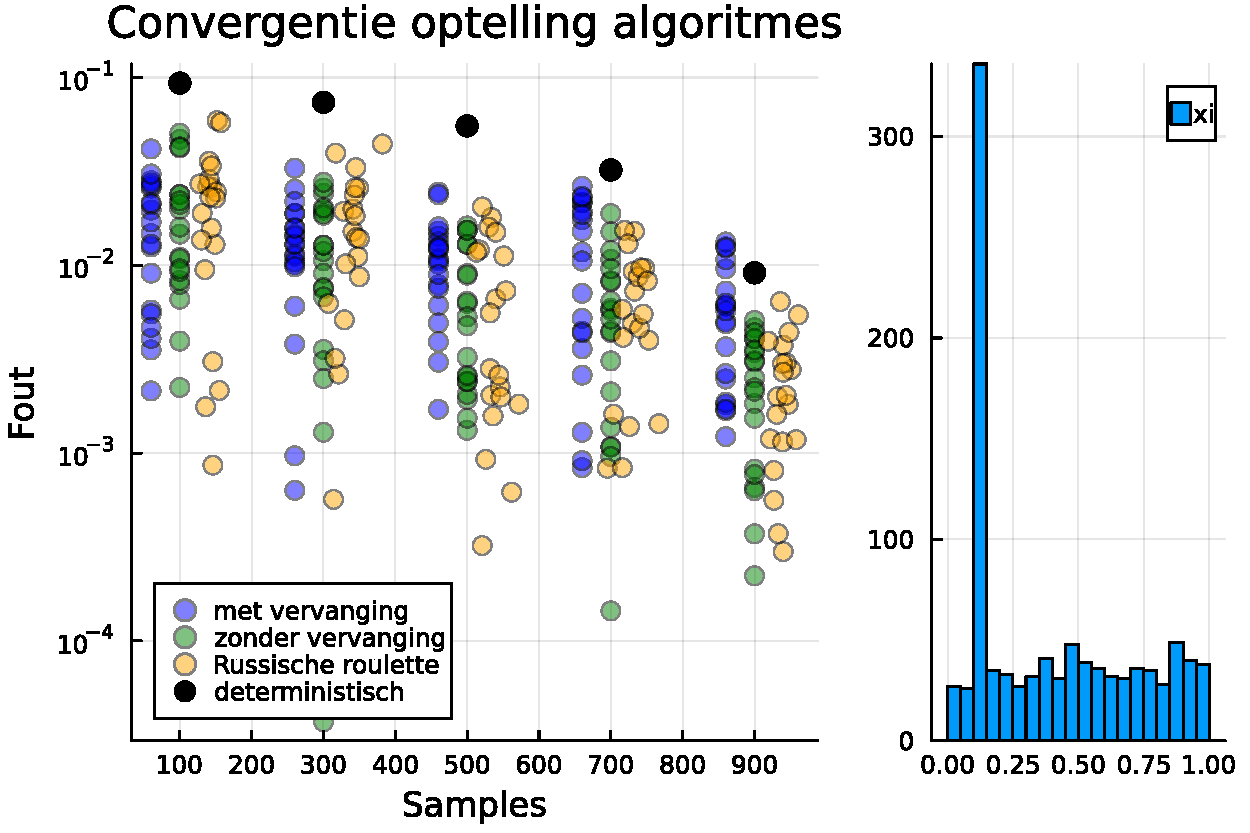
\includegraphics[width=0.8\textwidth]{imgs/convergence_sums.pdf}
        \label{fig:convergentie_optelling}
    \end{figure}
\end{frame}

\begin{frame}
    \frametitle{Main Poisson algoritme}

    \begin{align}
        \action<+->{y'                              & = A y + f \Leftrightarrow                                                              \\}
        \action<+->{y'+\sigma y                     & = (A + \sigma I) y + f\Leftrightarrow                                                                 \\}
        \action<+->{e^{-\sigma t} ( e^{\sigma t}y)' & = (A + \sigma I) y + f  \Leftrightarrow                                                               \\}
        \action<+->{y(t)                            & = e^{-\sigma t} y(0) + \int_{0}^{t} e^{(s-t) \sigma} \left(  (A(s) + \sigma I ) y(s) +f(s)\right) ds,}
    \end{align}
    \action<+->{doe volgende substitutie $e^{(s-t)\sigma} = \tau$, equivalent aan exponentieel te samplen}

    \begin{equation} \label{eq:poisson main}
        \action<+->{
        y(t) = \int_{0}^{e^{-\sigma t}}  y(0) d\tau
        + \int_{e^{-\sigma t}}^{1} \left(  \frac{A(s)}{\sigma} + I\right)  y(s) + \frac{f(s)}{\sigma} d\tau.
        }
    \end{equation}
    \action<+->{sample $\tau$ uniform, equivalent aan een Poisson proces te samplen.}
\end{frame}

\begin{frame}
    \frametitle{Main Poisson algoritme (recursief samplen)}

    \begin{equation} \label{eq:poisson main 2}
        y(t) = \int_{0}^{e^{-\sigma t}}  y(0) d\tau
        + \int_{e^{-\sigma t}}^{1} \left(  \frac{A(s)}{\sigma} + I\right)  y(s) + \frac{f(s)}{\sigma} d\tau.
    \end{equation}
    sample $\tau$ uniform, equivalent aan een Poisson proces te samplen. \\
    \action<+->{}
    \action<+->{
        Sample $y(t)$ recursief
        \begin{equation}
            Y(t)= \begin{cases}
                y(0)                                                               & \text{als }  e^{-\sigma t} \le  \tau \\
                \left(  \frac{A(S)}{\sigma} + I\right)  Y(S) + \frac{f(S)}{\sigma} & \text{anders}
            \end{cases}
            ,
        \end{equation}
        met $S = t +\frac{\ln\left(\tau\right)}{\sigma}$, let op $y \neq Y$
    }
\end{frame}

\begin{frame}
    \frametitle{Main Poisson algoritme (implementatie)}
    Verschillende implementaties, voorwaarts door Poisson proces andersom
    te samplen.
    \begin{figure}[h!]
        \centering
        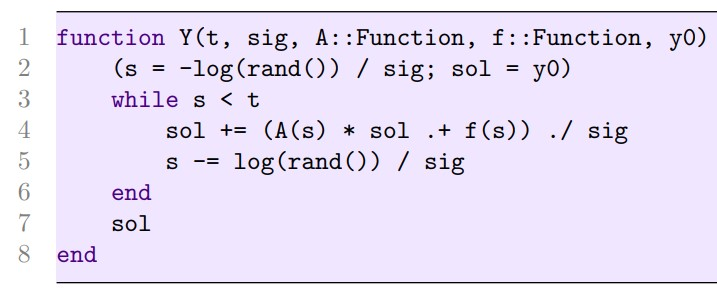
\includegraphics[width=0.8\textwidth]{imgs/main poisson julia.jpg}
        \label{fig:imgs/main poisson julia.jpg}
    \end{figure}
\end{frame}

\begin{frame}
    \frametitle{Main Poisson algoritme (convergentie)}
    Niet bewezen: robust tegen unbiased vervanging van $A,f,y(0)$.
    \begin{figure}[h!]
        \centering
        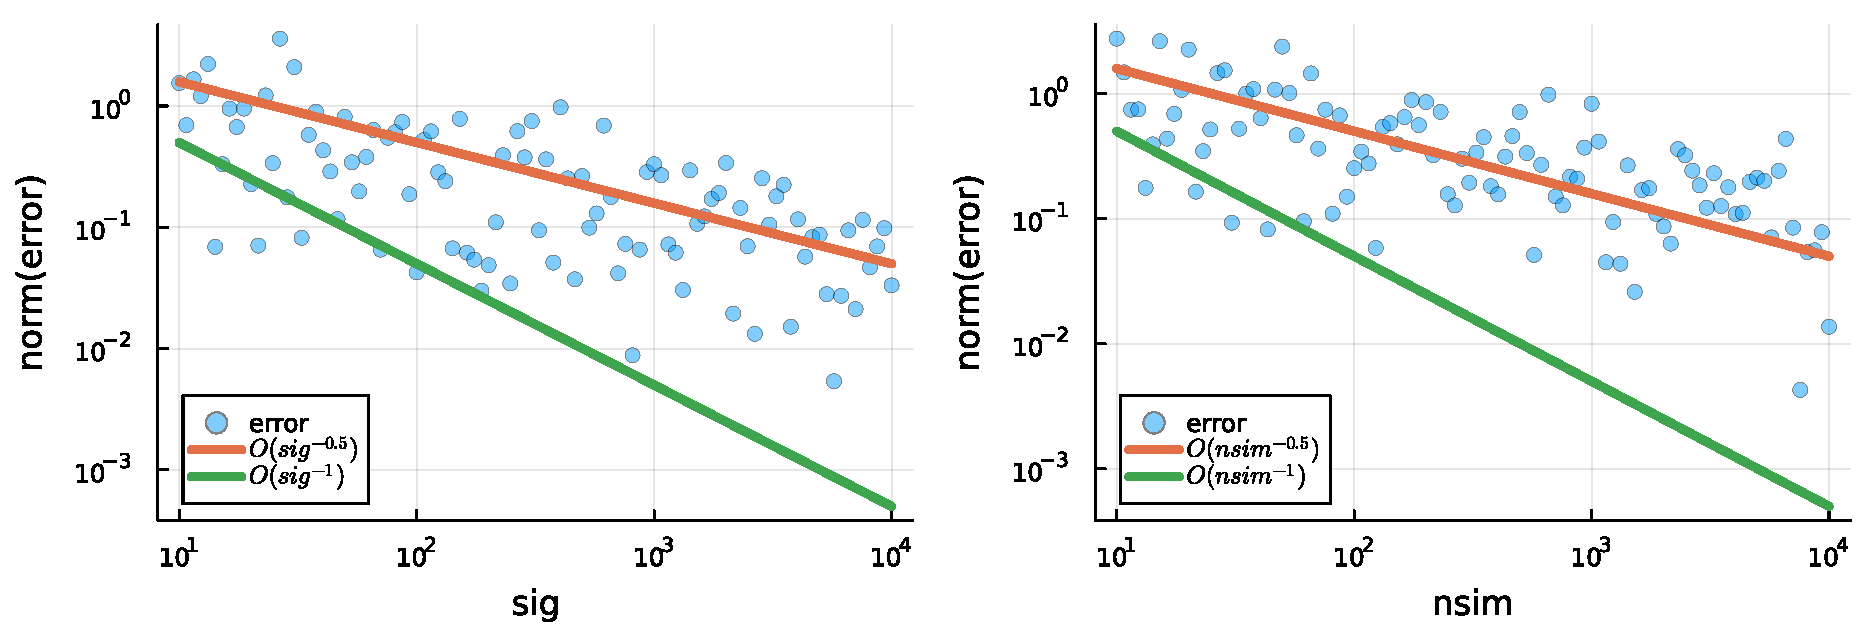
\includegraphics[width=\textwidth]{imgs/convergence_main_poisson.pdf}
        \caption{Realizaties van de norm van de fout,
            met $nsim =1$ en $\sigma$ variabel of $nsim$ variabel en $\sigma = 1$.
            Hoeveelheid samples van $A,f$ per simulatie $= \text{Poisson}(\sigma)$.
        }
        \label{fig:imgs/main poisson convergentie}
    \end{figure}
\end{frame}



\begin{frame}
    \frametitle{Limitaties}
    \begin{itemize}
        \item Stabiliteit $\rightarrow$ \cite{kettunen_unbiased_2021}
              (efficiënte unbiased $e^{\int A(s) ds } y(0)$ )
        \item Biased voor non-lineaire ODEs
    \end{itemize}
\end{frame}

\begin{frame}
    \frametitle{Toekomstig Werk}
    \begin{itemize}
        \item Random ODEs
        \item Specifieke ODEs
    \end{itemize}
\end{frame}

% 6 min
% \begin{frame}
%     \frametitle{Unbiased Non-Linearity}
%     \begin{itemize}
%         \item exponentiele voorbeeld + screenshot paper
%         \item VRE
%         \item Feynman-Kac formule
%         \item Magnus series
%     \end{itemize}
% \end{frame}

\end{document}